\documentclass[10pt,twocolumn,letterpaper]{article}

\usepackage{wacv}
\usepackage{times}
\usepackage{epsfig}
\usepackage{graphicx}
\usepackage{amsmath}
\usepackage{amssymb}
\usepackage{gensymb}

% Include other packages here, before hyperref.

% If you comment hyperref and then uncomment it, you should delete
% egpaper.aux before re-running latex.  (Or just hit 'q' on the first latex
% run, let it finish, and you should be clear).
%\usepackage[pagebackref=true,breaklinks=true,letterpaper=true,colorlinks,bookmarks=false]{hyperref}

\wacvfinalcopy % *** Uncomment this line for the final submission

\def\wacvPaperID{****} % *** Enter the wacv Paper ID here
\def\httilde{\mbox{\tt\raisebox{-.5ex}{\symbol{126}}}}

% Pages are numbered in submission mode, and unnumbered in camera-ready
\ifwacvfinal\pagestyle{empty}\fi
\setcounter{page}{1}
\begin{document}

%%%%%%%%% TITLE
\title{I-MOVE: Independent Moving Objects for Velocity Estimation}%, A RGB-D Dataset}

% Authors at the same institution
\author{Jonathan Schwan \hspace{2cm} Akshay Dhamija \hspace{2cm} Terrance E. Boult\\
University of Colorado, Colorado Springs\\
{\tt\small jschwan2@uccs.edu}
}

\maketitle
\ifwacvfinal\thispagestyle{empty}\fi

\maketitle

\begin{abstract}
\begin{quote}
  We introduce I-MOVE, a new public RGB-D dataset for estimating the velocity of a moving object. The dataset features various outdoor and indoor scenes of single moving objects where the position and velocity for the object is supplied. Compared to other datasets, a unique property is that the ground truth velocity for each of the moving objects has been calculated and included for a variety of different settings / environments and objects. The dataset includes training and test images that were captured from six different RGB-D camera views, the data is also time synchronized with additional equipment (radar, motion capture, etc.) to verify calculated velocity and position ground truth. There are approximately 600K training and 100K test images from each scene for each of the six RGB-D cameras. The I-MOVE dataset is available online at ???.com.
\end{quote}
\end{abstract}

\section{Introduction}
Motion parameter information is a necessary component in numerous applications. 
From robotic navigation, and collision detection to sport performance analysis, knowing an object's velocity is frequently needed \cite{kasiri2015combat,kasiri2017fine,wattanamongkhol2005method}. 
As more of these applications arise, the need grows for a computer vision based method to provide the appropriate motion parameter estimations \cite{marcon2010structural,miarka2011objectivity,polak2016motion}. 
Currently most motion parameter information has to be documented from devices on-board the moving object, such as IMUs (Inertial Measurement Unit) or via radars that are usually positioned knowing the object's path beforehand. 
In order to create a more useful and robust method to estimate motion parameters computer vision models are the logical next step.

\begin{figure}[t!]
    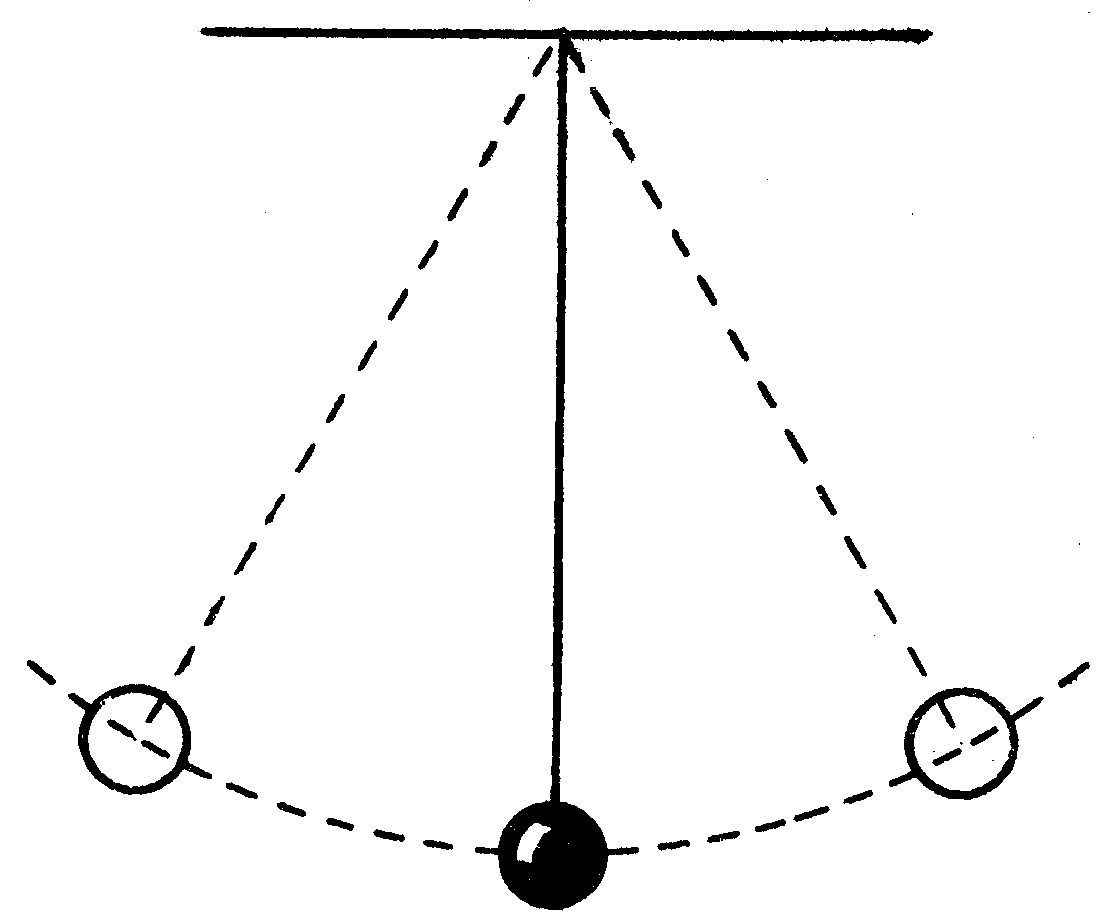
\includegraphics[width=1.0\columnwidth]{Images/pend.png}
    \caption{
    An example of the pendulum scene in the I-MOVE dataset.
    }\label{fig:pend.png} 
\end{figure}

In this paper, we introduce a new public RGB-D dataset to help address the above issues. 
The dataset features various outdoor and indoor scenes as opposed to most other RGB-D datasets which are frequently focused on static indoor environments. 
Our dataset also focuses on and provides annotations for a single moving object in each scene to best accommodate the greatest number of applications. 
The objects also vary though-out the scenes, for example some scenes are based upon a person's or dog's movements while others may be a rolling ball or pendulum as can be seen in Figure~\ref{fig:pend.png}. 


The main contribution of this dataset will be that each object's velocity will be provided in the ground truth. 
This allows people to train, test, and compare with the data. 
Taking another step to help bring the computer vision community closer to achieving accurate motion parameter estimation. 
The dataset includes training and test images that were captured from six different RGB-D camera views all time synchronized and with additional equipment (radar, motion capture, etc.) to verify calculated velocity and position ground truth. 
The camera type / model is also provided within the dataset. 
The cameras include: Three stereo setups of GoPro Hero 3s (six GoPros total), an Intel RealSense 435, Intel RealSense 415, and a ZED. 
This variety in devices helps to ensure the motion parameter estimation models will be as effective in the real world as possible.


\section{Motivation and Prior Works}
Vision-based velocity (or motion) estimation has been studied for decades. 
In recent years, as adequate cameras and computational power has become more accessible, the number of works attempting to estimate motion parameters has grown dramatically. 
Many of these works differ in the object and purpose for estimating motion parameters but all require a dataset with adequate ground truth and associate images.

From collision detection to athletic performance analysis, motion parameters are a crucial component to accuracy in these application. 
For example, to have an effective collision detection / time estimation model it is not only necessary to take into account your directional velocity but that of other objects. 
In order to accomplish this it is required that you have the three dimensional directional velocity of each of the objects within a reasonable view and distance.
Similarly, for object catching or throwing in the robotics field this information is essential to accurately estimating the trajectory / path of the object. 
For athlete performance analysis, numerous sports rely on velocity and acceleration information. 
Most obviously, sports where speed is the main component (running, biking, swimming, etc.), but also for sports such as weightlifting where the athletes are looking for their lift force and acceleration is required to calculate this, or for skateboarders attempting to add quantitative information to their training approach.

Prior attempts to estimate speed information in a relevant and accurate way have frequently relied on RGB-D data HERE


, where as those that used strictly RGB HERE


proved unreliable and too inaccurate to be plausible for real world applications. Due to the limited accuracy and possibility of successful estimations with purely RGB data or the existing RGB-D dataset, we found it necessary to create the I-MOVE dataset.

\section{Related Datasets}
First, we recognize the most similar datasets within the RGB-D realm. Then we address the most similar datasets in general intended to help work toward the solution to motion parameter estimation or a related task.

\subsection{RGB-D Datasets}
The most similar dataset within our knowledge is that mentioned in the paper, A Benchmark for the Evaluation of RGB-D SLAM Systems \cite{sturm_benchmark_2012}. The dataset contains the color and depth images of a Microsoft Kinect sensor along the ground-truth trajectory of the sensor. The ground-truth trajectory was obtained from a high-accuracy motion-capture system with eight high-speed tracking cameras in addition to accelerometer data from the Kinect. However, due to the extreme limitations of the Kinect and the fact that all of the data was collected indoors, with the same object, and without creation and validation of velocity data, there is significant need to create a more motion parameter estimation specific database.

The DIML RGB-D Dataset \cite{kim_deep_2018} also contains data collected with a Kinect, however this database does include indoor and outdoor video in addition to object segmentation making it more plausible to conduct tests upon for motion parameter estimation purposes.

\subsection{RGB or Motion Parameter Only Datasets}
The Human Activity Recognition dataset \cite{anguita_public_2013} provides potentially useful data to address the motion parameter estimation problem. The dataset contains smartphone accelerometer information collected by numerous people performing various tasks such as sitting, walking, and going up stairs. This dataset contains no images / video however and was created with the intention of being able to create a model that could predict the activity solely from the accelerometer information.

Another human activity recognition based dataset is the UTD-MHAD \cite{chen_utd-mhad:_2015} which is a dataset containing IMU and video information. This dataset contains 27 actions performed by 8 subjects (4 females and 4 males). Each subject repeated each action 4 times. The actions, such as knock on door, sit to stand, and stand to sit, are fairly limiting in movement, which make them not as desirable to estimate motion parameters for.

HumanEva is a synchronized video and motion capture dataset. The HumanEva dataset \cite{sigal_humaneva:_2010} consists of 4 subjects performing a set of six predefined actions three times (twice with video and motion capture, and once with motion capture alone). This dataset was intended to be used to improve upon existing three dimensional pose estimation but the information may also be used to train and test upon as motion parameter estimation models improve.

\section{The I-MOVE Dataset}
Compared to the reviewed datasets, I-MOVE is unique in a number of characteristics. 
Firstly the dataset is the only in our knowledge that focuses on and provides object motion parameters, it also contains a larger number of industry-relevant objects and scenes with both indoor and outdoor data to help provide adequate data to create more robust models. 
The data is also captured with a variety of cameras from six different angles in order to ensure accuracy in ground truth and maximum effectiveness when conducting tests of researcher's models. 
The velocity ground truth is also thoroughly proofed and tested to ensure accuracy with physics based examples and settings to allow completely mathematical based calculations to be done by hand and compared against. 

\subsection{Setup}
The equipment setup used for the dataset was meticulously crafted to ensure the most reliable results possible when setting up and collecting data in various locations / scenes. 
The six cameras and two radars were mounted on a 14 gauge angle bar as can be seen in Figure~\ref{fig:RIG.png}.

\begin{figure}[t!]
    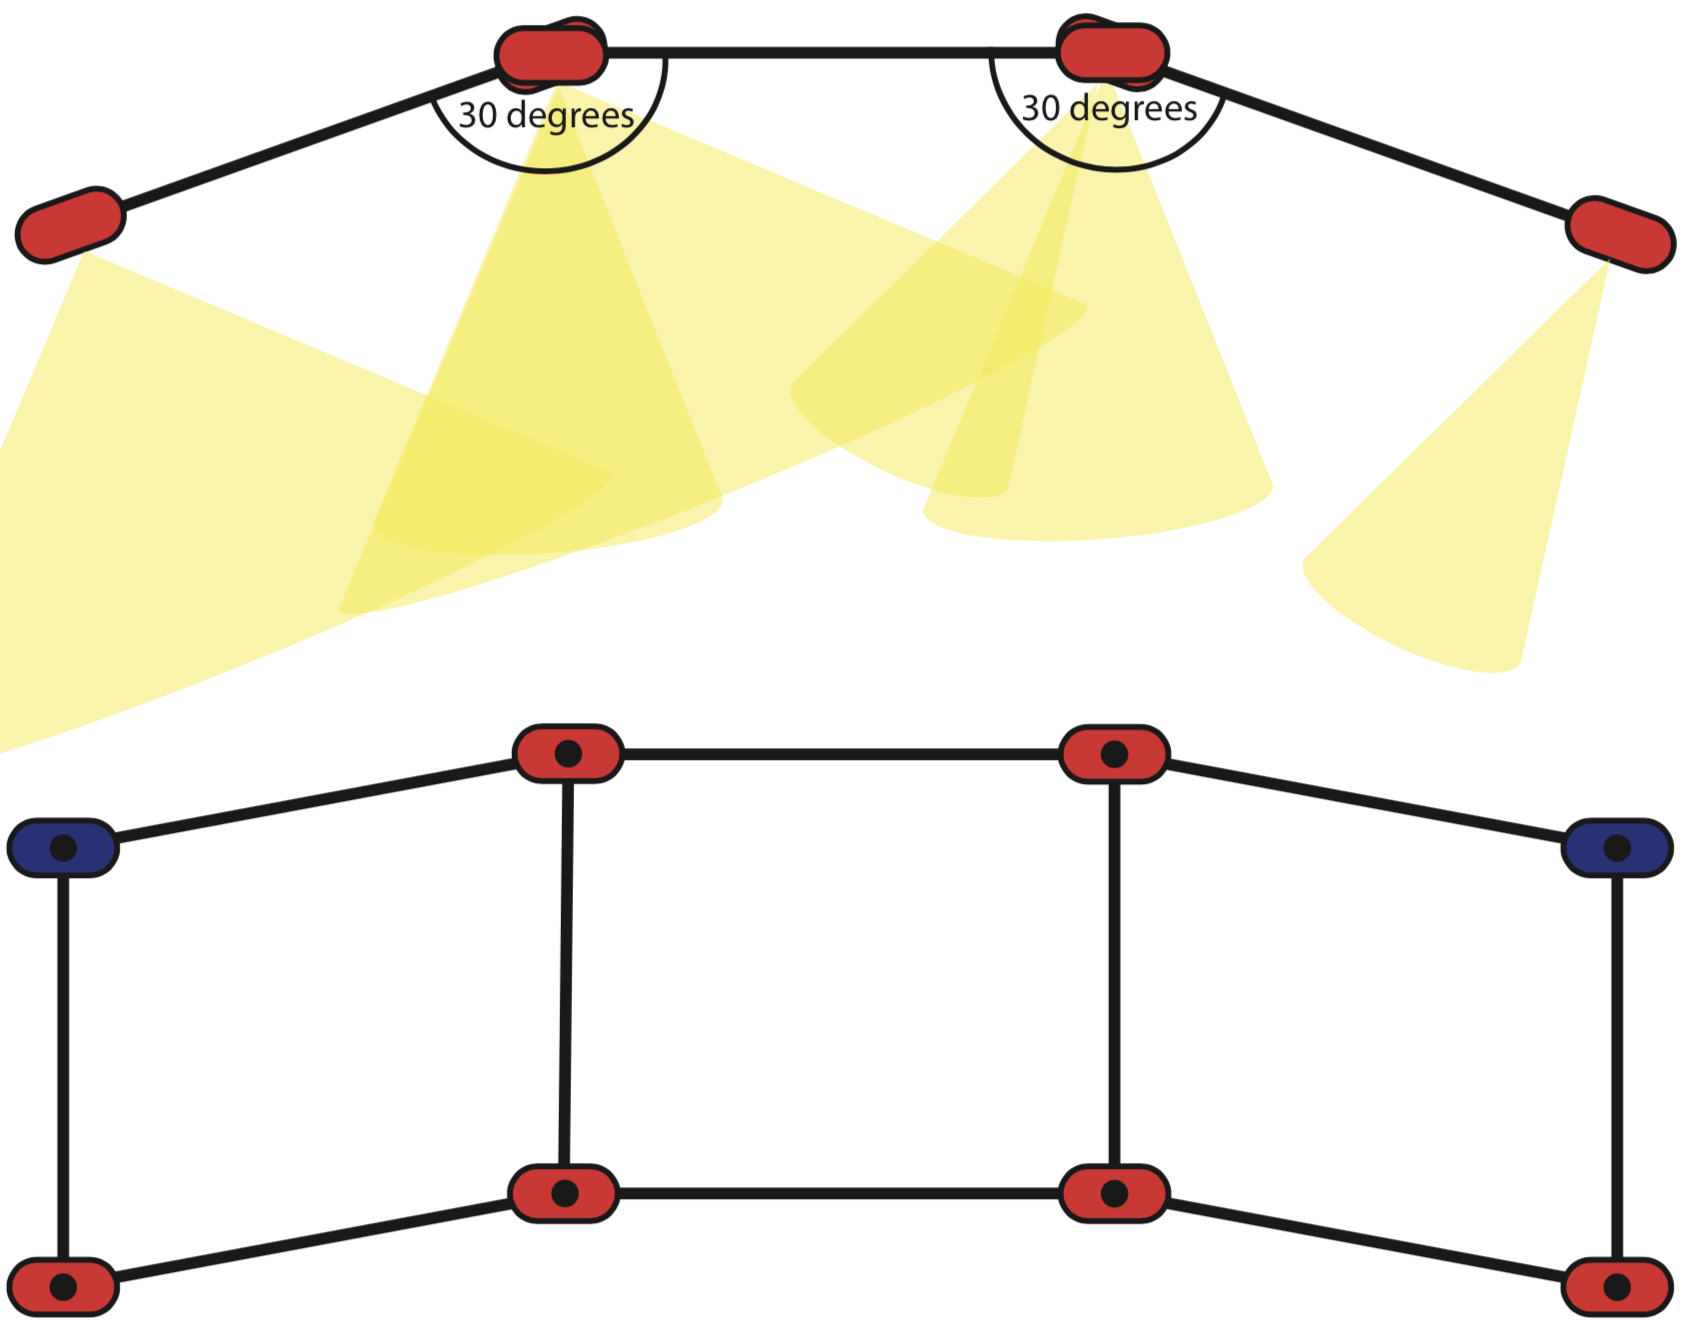
\includegraphics[width=\columnwidth]{Images/RIG.png}
    \caption{
    Above is the top view of the rig. each bar is 2 meters long and placed at a 30 degree difference from the other. The red rounded rectangles represent the cameras while the yellow represents the cameras' field of view. The field of view shrinks and pixel count increases as you go toward the right of the rig. The bottom is the front view of the rig as can be seen, there are six cameras represented by the red rounded rectangles and two radars represented by the blue rounded rectangles.
    }\label{fig:RIG.png} 
\end{figure}

The cameras and radars were mounted in the same order / setup for each location, to ensure appropriate comparisons can be made between different perspectives and camera effectiveness in different settings. 
The cameras used were three GoPro Hero 3 stereo rigs (six GoPros in total), along with two Intel RealSense cameras, a 415 and 435, and lastly a ZED camera. 
The radars used were OmniPreSense radars, which provide velocity of objects within their $78^{\circ}$ wide beams.

Due to the wide variety in lighting, size of objects and scene layouts / environments where data was collected the rig had to be created to accommodate these differences. 
The cameras all have a different degree of viewing capability so the order and spacing of them was vital to collect data as best possible. 
Two of the GoPro setups have modified lens giving them a field of view of $54.1^{\circ}$ for one of the modified setups and $64.7^{\circ}$ for the other.
The standard / unmodified GoPro stereo set up has a horizontal field of view of $122.6^{\circ}$.
The Intel RealSense 435 has a field of view of $85^{\circ}$ horizontally, while the RealSense 415 version has $63^{\circ}$, and finally, the ZED is capable of $90^{\circ}$ viewing horizontally.
Given our purposeful placement of the cameras we were able to obtain a two foot spacing between each camera allowing for fairly significant difference in camera perspective while still having all cameras capturing the object and it's most valuable movements. 
This can be seen in Fig ???

\subsection{Data Collection}
Our data collection process was intended to include a significant variety in objects, object motion, object velocity, scenes / environments and lighting, while still ensuring maximal accuracy in the ground truth for segmentation and velocity of the object.
The current dataset features ten different objects: person, car, dog, skateboarder, skateboard, biker, ball, drone, frisbee and RC Car. 
These objects differ widely not only in shape and size but also motion paths making them suitable to train and test upon. 

\subsection{Calculation and Verification of Velocity}
The main purpose of this dataset is to provide the necessary data to better predict motion parameters of an object. 
Because of this it is vital that the ground truth is as accurate as possible. 
To ensure the velocity of each object is correct we have additional purely physics based scenes put in place, some of these include dropping an object, rolling a ball down a ramp, and swinging a pendulum.
These can be seen in Figure\ref{fig:phys.png}

\begin{figure}[t!]
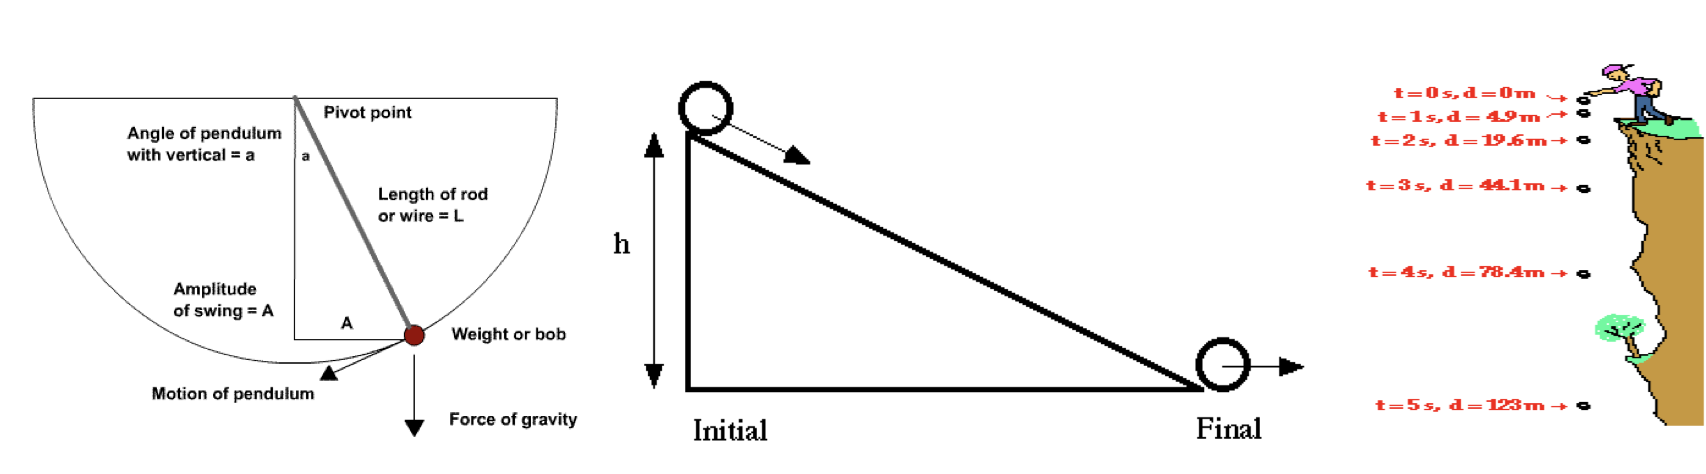
\includegraphics[width=\columnwidth]{Images/phys.png}
\caption{A schematic of the physics setups used for data collection. Pendulum seen on the left, rolling ball on incline in the middle, and dropping ball on the right.}\label{fig:phys.png} 
\end{figure}

The velocity data for the ball drop was computed using the commonly known equation $V = gt$ where gravity is 9.8 meters per second squared and t is the time since ball was released. The rolling ball's velocity at the end of the ramp / incline was calculated using the equation $V =  \sqrt{ \frac{10}{7}gh}$ where g is once again gravity and h is the height of the ramp. Finally the velocity of the pendulum was found using the equation $V =  \sqrt{2gL(1-cos(a)}$ where V is the velocity at the bottom of the swing, a is the angle from vertical, and L is length of the pendulum. These accompanied by hand calculated velocities using two OmniPreSense radars allow us to provide the most accurate velocities possible.

%\section{Segmentation Benchmark}

\section{Conclusion}
We present a novel dataset intended to help researchers progress and refine their approach and ability to produce more robust RGB-D object trackers for motion parameter estimation, specifically the velocity of the object being tracked with a meaningful metric. We identify several drawbacks, and limitations with the existing methods and datasets currently available for working on these problems in addition to explaining the differences between our dataset and ground truths. We explain how we derive and ensure accuracy in our bounding boxes / object segmentation and velocity of the object by using state of the art RGB-D object segmentation as our baseline and using commonly known physics equations and set-ups for several scenes. This dataset is also the first effort in our knowledge that directly approaches these problems and we intend to keep improving and expanding upon it.

In the future we plan to extend the dataset and labeling to contain more diverse settings, classes of objects as well as their motion paths and component / limb key points. We also hope to include additional motion parameters within the labeling such as angular velocity, and rotation in degrees. These additional motion parameters have the possibility of dramatically increasing the number of possible applications that a functioning motion parameter estimator could be applied to.


{\small
\bibliographystyle{ieee}
\bibliography{reu.bib}
}


\end{document}
